\week{There and Back Again}

Last week, we used data and rules to make our own interactive stories. These stories consisted of
a series of rooms. At each step, the reader of the story chose what to do next. Real-life computer
programs are structured in a similar way -- except, instead of a human player, the computer tells
itself what to do.

For example, imagine a story in which the user travels from town to town. The goal may be to
``travel to the next town''. At each step of the journey, perhaps it has the following actions that
could be done:

\begin{itemize}
    \item cross the bridge across the river
    \item take one step closer to the town
\end{itemize}

A player playing this would have to see what obstacles surrounded him and give directions to the
computer. If the player saw a river, he'd have to cross the bridge. If there was no river, then he
could just take the next step. At each step of the journey, there's only one choice for the next
step. Thus, this is a simple game to play and the player might get bored. However, even if it's
simple, the fact that there is a simple way to always pick the next step means that we can write a
program to play the game for us!\trythis{Think about how you'd describe the rules that would tell a
  computer how to play this game.}

Real life computer programs are often structured in this way. In fact, the way in which we've been
thinking about writing stories is one way in which computer scientists construct algorithms.

Just like moving from room to room in a story, real life computer programs \emph{move} from one set
of instructions to another.\hint{You're already familiar with what \emph{rooms} are in computer-speak -- functions!}

Think back a few weeks ago when we wrote programs that instructed DuckBot where to go, this would be
similar to a computer program playing one of the stories you wrote. Now think back to the some of
the issues we had with DuckBot: DuckBot sometimes ran in circles, sometimes it didn't cover the
entire pond and find the ducklings, and sometimes it simply crashed! All these outcomes are possible
when designing programs as well!

One key thing about our stories is that they all had endings. An ending could have been the player
succeeding, or it could have been the player failing. Either way, the stories eventually stopped --
but only if played correctly. Many of you had stories that allowed users to go back where they
started. If the user simply walked back and forth between rooms, or if you wrote a computer program
that did that, then the story would never end.

In this chapter, we will study one of the most powerful ideas in computer science, called
\term{recursion}. Recursion is what happens when a computer solves a problem by repeating a set of
instructions over and over again.

\curious{\textbf{What if a story never ended?}
Long ago, the Greek philosopher \emph{Zeno of Elea} imagined a strange situation. Suppose you are trying to
walk across a room. First, you must go halfway. Then, you must go halfway again. Then halfway again,
and again, forever. If there are always more halfway points to reach, how could you ever arrive? Try
opening the story \texttt{week6/zeno.py} and see if you can ever cross the room!

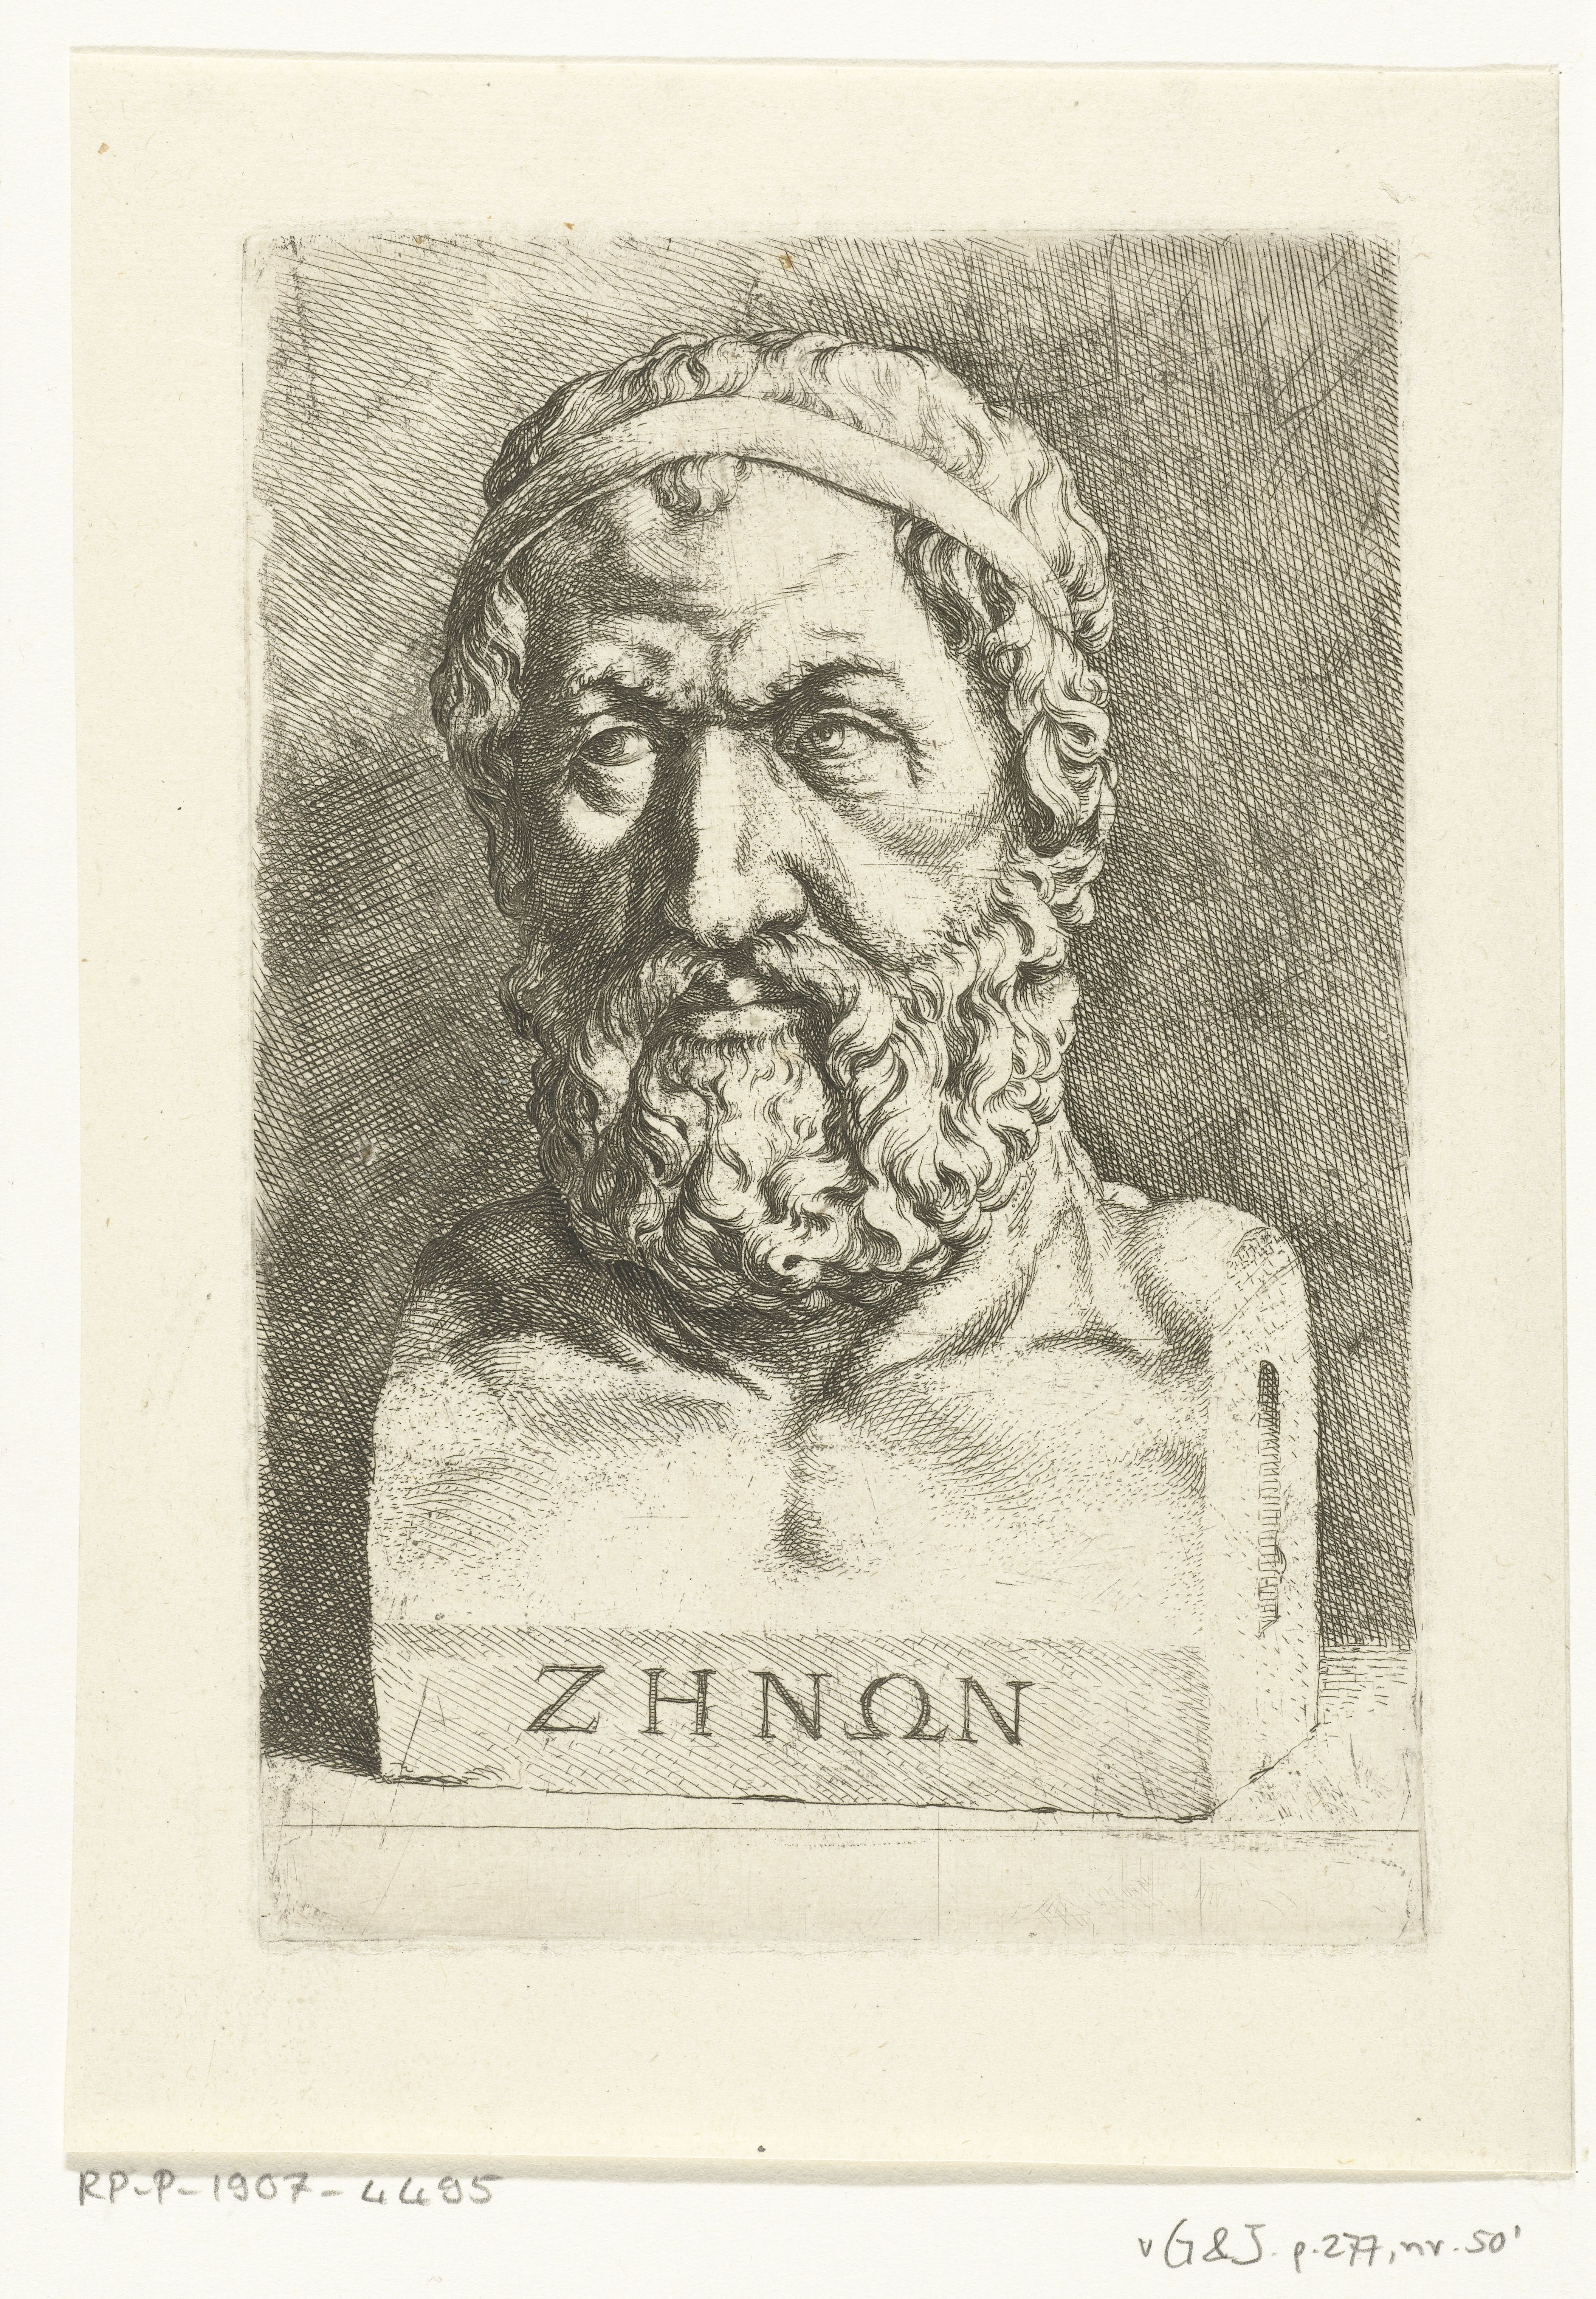
\includegraphics[width=0.9\marginparwidth]{../week6/figures/Zeno.jpg}}

\section{A Room That Leads to Itself}

In most of our stories so far, each room led to a \emph{different} room. The kitchen might have led
to the hallway, and the hallway to the corridor, and the corridor to the exit. Each step moved us
somewhere new.

Consider the following story: You are climbing a long staircase. You have limited energy. Going up
one step costs you one energy point. If you lose all energy points, you die. You must reach the top
of the stairs to win.

\begin{TryThisBox}
  Play this story right now by opening \texttt{week7/stairs.py} in Thonny and hitting the ``Run'' button.
\end{TryThisBox}

Take a look at this story and try playing it. Based on how it's written right now, would you ever be
able to win? What changes would you need to make to win this story? Go ahead and make those changes.

One of the key points of this story is that the \code{stairs} ``room'' leads to the
\code{next\_step} ``room,'' which leads back to \code{stairs}. This loop is the basis of
recursion.

\hint{Look at the two \kw{if} statements at the top of the \code{stairs} function.}
Now, you may think that in a story like this, there would be no way to escape. Once again, data
comes to the rescue. The story \emph{can} end, but only if \code{state} meets certain criteria. Can
you identify the two cases in which the story would end?

Without these two conditions, our story would go on forever without end! Because these two stories
``end'' the loop, we call them \term{base cases}. Without \term{base cases}, recursion goes on
forever.\curious{Think back to DuckBot, and the times DuckBot swam in circles forever. Knowing what
  we know now, this is because the \term{base cases} for DuckBot's behaviors were wrong}

To summarize, every recursive program needs (1) a way to continue and (2) a way to stop. Once we
have these, we can use recursion to solve problems.

\section{Searching}

The staircase story showed us one kind of recursion: each time we made a move, we returned to the
same story, but with a slightly different \code{state}. That is already a powerful idea. But
recursion becomes even more useful when it helps us solve a real problem more \emph{efficiently}.

\trythis{You can play this story by opening up \texttt{week7/search.py} in Thonny.}
Suppose you are trapped in a tower with many numbered rooms. The room numbers are all written in
order, from smallest to largest. Somewhere in this list is the goal room. Your task is to find it.

One way to search would be to check the rooms one by one. But here's the catch: just like with the
stairs story, you only have a limited number of steps you can take.

You are given several choices. You can go \code{one up} or \code{one down}, checking rooms one at
a time. But you can also try something more ambitious: you can move \code{halfway up} or
\code{halfway down}, jumping across the tower in larger steps.

At first, this seems like a very powerful ability. If the goal room has a larger number, why not
jump halfway up? If it has a smaller number, why not jump halfway down? It feels like you should be
able to find the goal very quickly.

\begin{TryThisBox}
  Try playing the story, and completing it using \code{go halfway up} and \code{go halfway down}. Is
  it always possible to find the room? Why or why not?
\end{TryThisBox}

You've probably noticed that both strategies don't quite work. Even when taking the ``big'' steps,
you sometimes overshoot and go past your goal.

In order to understand, we have to pay attention to what the story remembers and what it doesn't.

Each time you move, the story tells you whether the goal is larger or smaller than the current
room. That means you are learning something important with each step. For example, if the goal is
larger than the current position, then you now know that \emph{every room below your current
position cannot be the goal.}

But what does the program do with this information? Absolutely nothing right now.

Even after learning that half of the rooms are impossible, the story continues to treat the entire
list of rooms as if they were still possible. It moves around the tower, but it never truly
\emph{narrows down} the search.

This is the key problem: at each recursive step, the full list of rooms are still being considered,
even though we know some of them are impossible. In other words, the list of rooms never shrinks.

\hint{You'll have to modify the \code{one\_up} and \code{one\_down} functions to change the ``top'' and ``bottom'' rooms.}
\begin{TryThisBox}
  Your task now is to fix this program so that the list of rooms ``shrinks'' each time the user decides
  to go halfway up or halfway down.
\end{TryThisBox}

If you've made the fix properly you should always be able to find the room in the allowed number of steps.

\subsection{How many steps?}

When we played DuckBot, we asked how many \kw{if} statements we needed to tell DuckBot what to
do. This is one way of measuring how complicated a program is. Another way of measuring how
complicated a program is is figuring out how many ``steps'' it takes. In our case, we started with
32 rooms. If we only could use the single step directions, then we would need up to 32 steps in
order to find any room. But since we had the halfway directions, we only needed five.

How many steps would it take to find a room in a 10,000 room tower?

\hint{You can go ahead and try to play the game with 10,000 rooms by modifying the \code{room\_count} variable at the end of the file.}
One way to understand this is realizing that everytime we take a halfway step, we reduce the total
number of rooms we could enter by half. So we really want to know how many times we can half 10,000?
\[
\begin{array}{|l|l|}
\hline
\text{Step 1:} \, \frac{10000}{2} = 5000 & \text{Step 2:} \, \frac{5000}{2} = 2500 \\
\hline
\text{Step 3:} \, \frac{2500}{2} = 1250 & \text{Step 4:} \, \frac{1250}{2} = 625 \\
\hline
\text{Step 5:} \, \frac{625}{2} \approx 312 & \text{Step 6:} \, \frac{312}{2} = 156 \\
\hline
\text{Step 7:} \, \frac{156}{2} = 78 & \text{Step 8:} \, \frac{78}{2} = 39 \\
\hline
\text{Step 9:} \, \frac{39}{2} \approx 19 & \text{Step 10:} \, \frac{19}{2} \approx 9 \\
\hline
\text{Step 11:} \, \frac{9}{2} \approx 4 & \text{Step 12:} \, \frac{4}{2} = 2 \\
\hline
\text{Step 13:} \, \frac{2}{2} = 1 & \\
\hline
\end{array}
\]

So, we would need thirteen steps. This is more than twice the number of steps we needed for a
32-room tower. But notice that 10,000 is about 300 times larger than 32, yet we only need about twice
as many steps for a 10,000 room tower.

This is the power of recursion. Because we halfed the problem size at each step, we only need to
take a handful of steps to find any room. \prettyref{tab:logarithms} gives the maximum number of
steps we'd need to take for towers in a wide variety of sizes. Notice that even for towers
containing \emph{billions} of rooms, we still need just a few steps!

\begin{table}[ht]
    \centering
    \caption{Maximum Number of Steps Needed for Various Tower Sizes Using Binary Search. Note that $10^{n}$ means a $1$ followed by $n$ zeros.}
    \label{tab:logarithms}
    \begin{tabular}{|c|c|}
        \hline
        \textbf{Number of Rooms} & \textbf{Maximum Steps} \\
        \hline
        1 & 0 \\
        2 & 1 \\
        4 & 2 \\
        8 & 3 \\
        1,024 & 10 \\
        1,048,576 & 20 \\
        1,073,741,824 & 30 \\
        $10^{15}$ & 50 \\
        $10^{30}$ & 100 \\
        $10^{80}$ (approx \# of particles in the universe) & 265 \\
        \hline
    \end{tabular}
\end{table}
